\documentclass[11pt]{beamer}
\usetheme{OIE}
\usepackage[utf8]{inputenc}
\usepackage[german]{babel}
\usepackage[T1]{fontenc}
\usepackage{amsmath}
\usepackage{amsfonts}
\usepackage{amssymb}
\usepackage{tikz}
\usepackage{graphicx}
\usepackage{color}
\usepackage{booktabs}
\usepackage{pifont}
\usepackage{xcolor}
\usepackage{fancyvrb}
\usepackage[natbib=true,backend=bibtex,style=authoryear]{biblatex}
\author{Dominik Both, Tonio Weidler}
\title{Open Information Extraction}
%\setbeamercovered{transparent} 
%\setbeamertemplate{navigation symbols}{} 
%\logo{} 
\institute{Institut für Computerlinguistik, Universität Heidelberg} 
\date{15.07.2016} 
\subject{} 
\definecolor{lightgray}{gray}{0.8}

\begin{document}

% AUTOMATISMEN
\AtBeginSection{\frame{\sectionpage}}
\AtBeginSubsection{\frame{\subsectionpage}}


% TEMPLATING
\setbeamertemplate{title page}{
	\center 
		\begin{beamercolorbox}[center]{part title}
	      \Huge\inserttitle\par
	    \end{beamercolorbox}
	    \vspace{15pt}
		\insertauthor\\
		\vspace{15pt}		
		Proseminar \textit{Text Mining}\\
		Andrea Zielinski\\
		\vspace{15pt}
		\insertinstitute, \insertdate
}

\defbeamertemplate{section page}{wiqe}[1][]{%
  \begin{centering}
    \begin{beamercolorbox}[center]{part title}
      \Huge\insertsection\par
    \end{beamercolorbox}
  \end{centering}
}

\defbeamertemplate{subsection page}{wiqe}[1][]{%
  \begin{centering}
    \begin{beamercolorbox}[center]{}
      \usebeamerfont{subsection title}\usebeamercolor[fg]{subsection name}\insertsection\par
    \end{beamercolorbox}
    \begin{beamercolorbox}[sep=2pt,center]{part title}
		\huge\insertsubsection\par
    \end{beamercolorbox}
  \end{centering}
}
\setcounter{tocdepth}{1}
\setbeamertemplate{section page}[wiqe]
\setbeamertemplate{subsection page}[wiqe]

% COMMANDS
\newcommand{\hitem}{
	\item[\color{lightgray}\rule{0.5em}{0.5em}]
}

\begin{frame}
\titlepage
\end{frame}

\begin{frame}{Papers}

Identifying Relations for Open Information Extraction (Fader et al., 2011)\\
\vspace{15pt}
LODifier: Generating Linked Data from Unstructured Text (Augenstein et al., 2012)

\end{frame}

\begin{frame}{Strukturierung}
    \tableofcontents
\end{frame}

\section{Introduction to Information Extraction}
	\begin{frame}{What is Information Extraction?}
			\begin{center}
			\begin{block}{Information Extraction}
				Goal of Information Extraction is automatically extracting information from unseen text\\
				\textit{Information:} entities, relations, events...\\
				\end{block}
				\vspace{15pt}
				To make the dough for a good pizza, we start with putting 1kg of flour into the mixing bowl.\\
				\textit{(1kg of flour, put into, mixing bowl)}
			\end{center}
	\end{frame}
	\begin{frame}{Problems of Information Extraction}
				\begin{center}
				\begin{itemize}
					\item Named Entity Recognition
					\item Relationship Extraction 
					\item Coreference Resolution
					\item Comment Extraction
					\item many more..
					\end{itemize}
				\end{center}
	\end{frame}
\section{OIE - Principles}
	\subsection{Open Information Extraction}
		\begin{frame}{Open Information Extraction}
			\begin{center}
				
				\textit{IE:} Extractor for each target relation\\
				\vspace{10pt}
				\textit{Open:} No pre-specified extractors\\
				\vspace{10pt}
				Unsupervised learning of relation phrases\\
				\vspace{10pt}
				Extraction of information on every given domain

			\end{center}
		\end{frame}
		\begin{frame}{Problems of Open Information Extraction}
					\begin{center}
						\begin{itemize}
						\item \textbf{Incoherent extractions:}\\
							This guide contains dead links and omits sites
							\\\textit{contains omits}
						\item \textbf{Uninformative extractions:}\\
							Faust made a deal with the devil
							\\ \textit{(Faust, made, a deal)}
						\end{itemize}
					\end{center}
				\end{frame}
	\subsection{Methods}
		\begin{frame}{Text Runner and WOE}
			\begin{center}
				\begin{enumerate}
				\item \textit{Label:} Automatic sentence labeling by heuristics
				\item \textit{Learn:} A relation phrase extractor is learned
				\item \textit{Extract:} Identifying NP pairs and searching relations words between
				\end{enumerate}
			\end{center}
		\end{frame}
		\begin{frame}{Problems}
					\begin{center}
						\begin{itemize}
						\item Large number of labeled training examples required
						\item Alternative heuristic labeling leads to huge noise and stacked uncertainty
						\item Ignores both holistic and lexical aspects 
						\end{itemize}
					\end{center}
				\end{frame}
		
		
		\begin{frame}{Syntactic constraint}
			\begin{center}
				\begin{itemize}
				\item Limits relations to those matching a certain POS Tag pattern:
				\item V | V P | VW* P %ich mache dann Beispiele was das heißt
				\item Always choses longest possible match
				\item Merge ajacent matches together
				\end{itemize}
				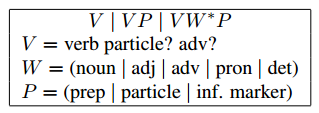
\includegraphics[scale=1.5]{img/pos.png}\\
				%beispiel mit faust
			\end{center}
		\end{frame}
		\begin{frame}{Lexical constraint}
			\begin{center}
				\begin{itemize}
				\item Only assume relations that appear in the corpus for a certain amount
				\item The Obama administration \textbf{is offering only modest greenhouse gas reduction targets at} the conference
				\end{itemize}
			\end{center}
		\end{frame}
		\begin{frame}{Limitations of those constraints}
			\begin{center}
				\begin{itemize}
				\item In a set of 300 hand-annotated sentences 85\% relations fell into those constraints
				\item Model is not complete and has its flaws
				\end{itemize}
				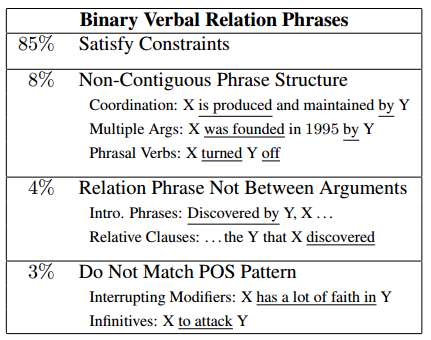
\includegraphics[scale=0.7]{img/constraints.png}\\	
			\end{center}
		\end{frame}
		\begin{frame}{ReVerb Extraction Algorithm}
			\begin{center}
				\begin{itemize}
				\item \textit{Relation Extraction: }Find the longest possible string of words that match the relation constraints, merge adjacents
				\item \textit{Argument Extraction:} Find the nearest NP left and right to the relation that is not a relativ pronoun, WHO-adverb or existential-there.
				\item How is the lexical constraint being checked? By creating a list of relational phrases by applying this algorithm on a 500 million Web sentences.
				\end{itemize}
			\end{center}
		\end{frame}
		\begin{frame}{ReVerb Confidence Function}
					\begin{center}
						\begin{itemize}
						\item The Algorithm has a high recall, but low precision
						\item Now the extracted relation is weighted by a confidence function:
						\end{itemize}
						
					\end{center}
				\end{frame}
				\begin{frame}{ReVerb Confidence Function}
					\begin{center}
						
						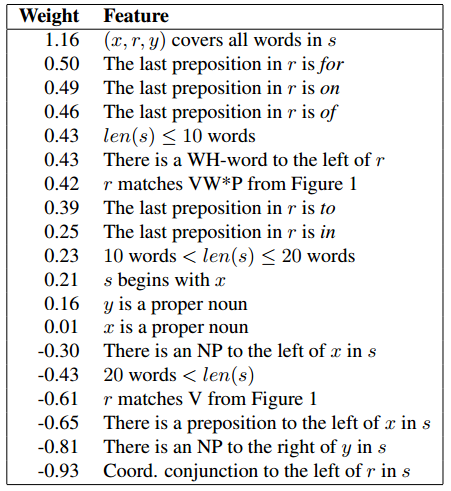
\includegraphics[scale=0.8]{img/sososo.png}\\
					\end{center}
				\end{frame}
				\begin{frame}{Evaluation}
					\begin{center}
						
						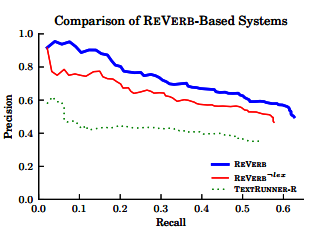
\includegraphics[scale=0.8]{img/reverbeval.png}\\
						Better results than TextRunner through lexical features, but still low recall.
					\end{center}
				\end{frame}
				\begin{frame}{Why?}
					\begin{center}
						
						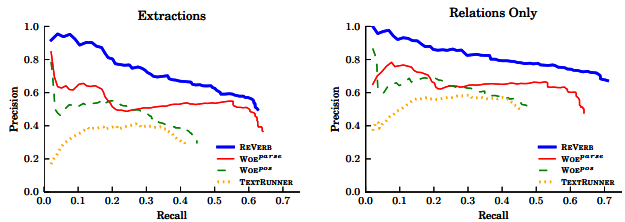
\includegraphics[scale=0.7]{img/reverbeval2.png}\\
						Argument extraction is open to improvements
					\end{center}
				\end{frame}
				\begin{frame}{Why?}
					\begin{center}
						Evaluating the evaluation: 
						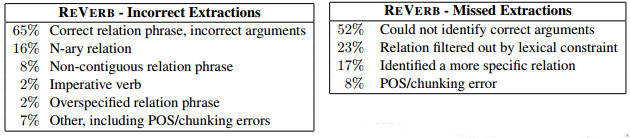
\includegraphics[scale=0.7]{img/reverberrortypes.png}\\
						
					\end{center}
				\end{frame}
				\begin{frame}{Conclusion}
					\begin{center}
						
						
					\end{center}
				\end{frame}
	\subsection{Data Representation}
		\begin{frame}{Standard Patterns}
			\begin{center}
				\includegraphics[scale=0.5]{img/oie-pattern.png}\\
				\vspace{15pt}
				\textbf{Argument A} is in a directed \textbf{relation} to \textbf{Argument B}.
			\end{center}
		\end{frame}
		
		\begin{frame}{Unnormalized Annotation}
			\begin{center}
				(argument\_a, predicate\_x, argument\_b)\\
				(argument\_a, predicate\_y, argument\_c)\\
				(argument\_a, predicate\_y, argument\_d)
			\end{center}
			\vspace{15pt}
			\textbf{Problems}\\
			\begin{itemize}
				\item redundant
				\item unnormalized
				\item can only produce binary predicates
			\end{itemize}
		\end{frame}
		
		\begin{frame}{RDF and Linked Data}
			\begin{block}{Resource Description Framework}
				Models propositions by constructing \textit{triples} including \textbf{Subjects}, \textbf{Objects} and \textbf{Predicates}\\
				Generates a directed graph
			\end{block}
			\vspace{10pt}
			\begin{center}
				:subject :predicate :object.
				\vspace{10pt}
				\includegraphics[scale=0.5]{img/oie-rdf-triple.png}
			\end{center}
		\end{frame}
		
		\begin{frame}{RDF Concepts and Notation}
			\begin{itemize}
				\item \textbf{URIs}\\
					identifies ressources (S, R, O) distinctivly and references further informations (triples)
				\item \textbf{Conclusions}\\
					allows to draw conclusions using rules
				\item \textbf{Turtle}\\
					allows syntax abbreviations
				\item \textbf{Blanknodes}\\
					placeholder for something without a URI
				\item \textbf{Queries}\\
					can be searched by querying (eg SPARQL)
				
			\end{itemize}
		\end{frame}
		
		\begin{frame}{RDF Reification}
			\textbf{Motivation:} How can I realize embedded propositions?\\
			\vspace{10pt}
			\textbf{Example:} Peter said, he watched the movie.\\ 
			\vspace{15pt}
			
			\only<2>{
			\textbf{Wrong proposition}
			\begin{center}
				:Peter :watched :movie
			\end{center}
			}
			
			\only<3>{
			\textbf{Reification}\\
			\begin{center}
				\begin{tabular}{l}
					:Peter :said \_:prop.\\
					\_:prop rdf:subject :Peter.\\
					\_:prop rdf:predicate :watched.\\
					\_:prop rdf:object :movie. \\
				\end{tabular}
			\end{center}
			}
			
		\end{frame}
		
		\begin{frame}{Vocabularies \& Ontologies}
			Several vocabularies provide useful relations and functionality, eg.:
			\begin{itemize}
				\item RDF (rdf:type, ...)
				\item RDFS (rdfs:subClassOf, rdfs:domain, rdfs:range, ...)
				\item OWL (owl:sameAs, owl:SymmetricProperty, ...)
				\item FOAF
			\end{itemize}
			
			Ontologies are huge RDF Graphs containing many triples, eg.:
			\begin{itemize}
				\item DBpedia
				\item Wikidata
				\item WordNet
			\end{itemize}						
		\end{frame}
		
		\begin{frame}[fragile]{RDF Syntax}
			\begin{verbatim}
				dbr:Barack_Obama a foaf:person, :President;
				    dbo:spouse dbr:Michelle_Obama.
				dbr:Bernie_Sanders dbo:birthPlace dbr:New_York, 
				                                  dbr:Brooklyn;
				dbr:Brooklyn dbo:isPartOf dbr:New_York 	
			\end{verbatim}
		\end{frame}
		
		\begin{frame}{... as Graph}
			\begin{center}
				\includegraphics[scale=0.4]{img/oie-rdf-example.png}
			\end{center}			
		\end{frame}

\section{Example: LODifier}
	\begin{frame}{LODifier: Generating Linked Data from Unstructured Text (Augenstein et al., 2012}
		\begin{center}
			Generate an RDF Graph from unstructured Text\\
			\vspace{15pt}
			\textbf{Past Approaches:} Use Patterns to trade recall for precision\\
			\textbf{LODifier:} Process the entire text
		\end{center}
	\end{frame}
	\subsection{Architecture}
		\begin{frame}{Architecture}
			\begin{center}
				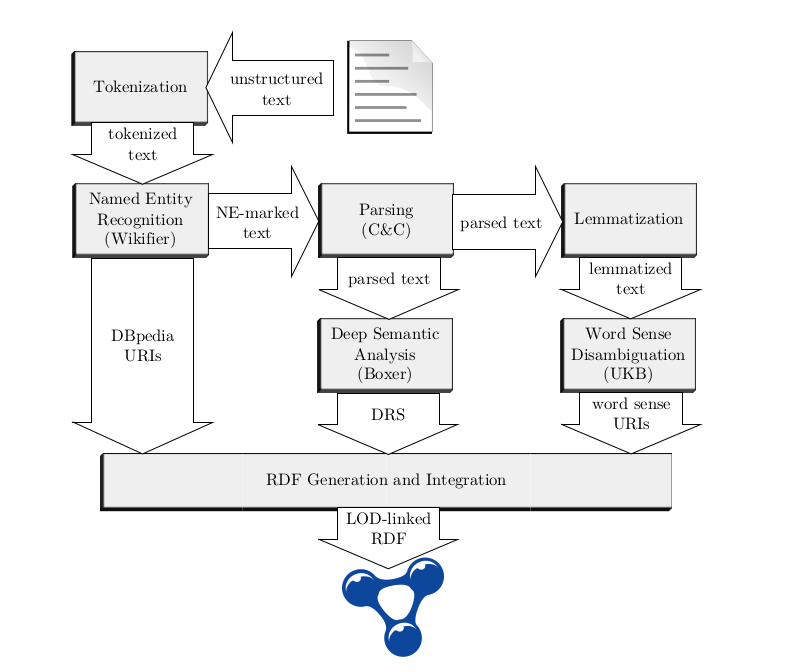
\includegraphics[scale=0.25]{img/oie-lodifier-architecture.png}
			\end{center}
		\end{frame}
		
		\begin{frame}{Approach}
			\begin{enumerate}
				\item \textbf{Parse} the input text (POS, Treetagging, NER)
				\item Apply \textbf{Deep Semantic Analysis} to get relations
				\item Enrich NEs and words with \textbf{URIs} (DBpedia and WordNet)
				\item Forge an \textbf{RDF Graph} of this information
			\end{enumerate}					
		\end{frame}
		
		\begin{frame}{How does it happen?}
			Lets go through the process step-by-step!\\
			\vspace{15pt}
			\textbf{Example Text:}\\
			The New York Times reported that John McCarthy died. He invented the programming language LISP.\\
			\tiny{example taken from Augenstein et al., 2012}			
		\end{frame}
	\subsection{Preprocessing}
		\begin{frame}{Named Entity Recognition - Wikifier}
			\begin{block}{Wikifier}
				Recognizes NE and replaces them with the Wikipedia Page Link\\
				Disambiguates by comparing links between pages.
			\end{block}
			\vspace{15pt}
			\textbf{Example Text Output:}\\
			\textcolor{green}{[The New York Times]} reported that \textcolor{green}{[John McCarthy (computer scientist)|John McCarthy]} died. He invented the \textcolor{gray}{[Programming language|programming language]} \textcolor{gray}{[Lisp (programming language)|LISP]}.
		\end{frame}
		
		\begin{frame}{Parsing Syntax - C\&C}
			\begin{block}{C\&C Parser}
				Syntactical Parser that tags POS and builds Parse Trees in CCG.
			\end{block}
			
			\begin{block}{Combinatory Categorial Grammar (CCG)}
				Grammatical formalism allows parallel analysis of syntax and semantics\\
				Associates words with categories that can be combined (rule-based) to form a sentence\\
				Syntax via Category Combination, Semantics via lambda calculus
			\end{block}
		\end{frame}
		
		\begin{frame}[fragile]{Parsing - Output}
			\begin{Verbatim}[fontsize=\tiny]
				ccg(1, rp(s:dcl,
				    ba(s:dcl,
				      lx(np, n,
				        t(n, ’The_New_York_Times’, ’The_New_York_Times’, ’NNS’, ’I-NP’, ’O’)),
				      fa(s:dcl\np,
				        t((s:dcl\np)/s:em, ’reported’, ’report’, ’VBD’, ’I-VP’, ’O’),
				        fa(s:em,
				          t(s:em/s:dcl, ’that’, ’that’, ’IN’, ’I-SBAR’, ’O’),
				          ba(s:dcl,
				           lx(np, n,
				             t(n, ’John_McCarthy’, ’John_McCarthy’, ’NNP’, ’I-NP’, ’I-PER’)),
				           t(s:dcl\np, ’died’, ’die’, ’VBD’, ’I-VP’, ’O’))))),
				    t(period, ’.’, ’.’, ’.’, ’O’, ’O’))).				
				ccg(2, rp(s:dcl,
				    ba(s:dcl,
				      t(np, ’He’, ’he’, ’PRP’, ’I-NP’, ’O’),
				      fa(s:dcl\np,
				        t((s:dcl\np)/np, ’invented’, ’invent’, ’VBD’, ’I-VP’, ’O’),
				        fa(np:nb,
				          t(np:nb/n, ’the’, ’the’, ’DT’, ’I-NP’, ’O’),
				          fa(n,
				            t(n/n, ’programming_language’, ’programming_language’, ’NN’, ’I-NP’, ’O’),
				            t(n, ’LISP’, ’LISP’, ’NNP’, ’I-NP’, ’O’))))),
				    t(period, ’.’, ’.’, ’.’, ’O’, ’O’))).
			\end{Verbatim}
		\end{frame}
		
		\begin{frame}{Find Relations - Boxer}
			\visible<1-3>{\begin{block}{Boxer}
				Creates DRSs from C\&C Output
			\end{block}}

			\visible<2-3>{\begin{block}{Discours Representation Structure (DRS)}
				Represents the discourse via \textit{relations} between \textit{entities}\\
				Allows referencing over the entire discourse
			\end{block}}
			
			\visible<3>{
				\vspace{5pt}
				\textbf{Boxers DRS Relations (Conditions):}\\
				\begin{itemize}
					\item \textbf{Unary Relations (Classes):} eg. \textit{topic}, \textit{person}, \textit{event}, \textit{male}, ... + all verbs
					\item \textbf{Binary Relations:} agent, patient, ... (semantic roles)
				\end{itemize}							
			}
		\end{frame}	
				
		\begin{frame}{Boxer Output}
			\begin{center}
				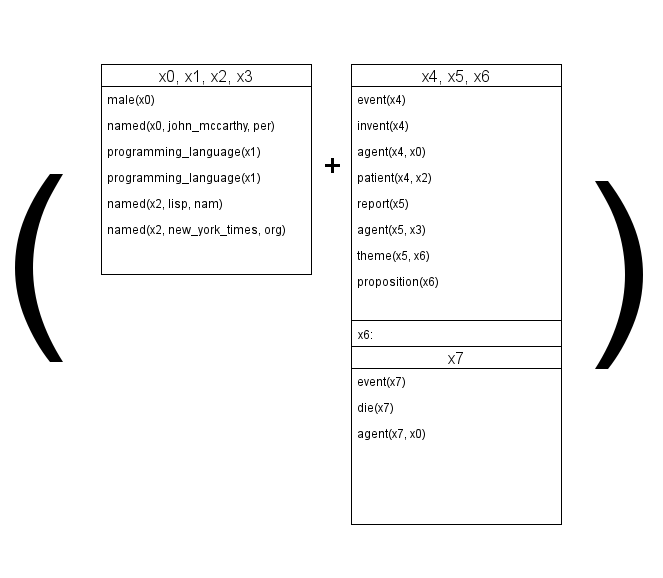
\includegraphics[scale=0.3]{img/oie-boxer-output.png}
			\end{center}
		\end{frame}
		
		\begin{frame}{Assign WordNet URIs}
			\begin{block}{RDF WordNet}
				\textbf{WN:} Lexicography containing senses linked by semantic relations\\
				\textbf{RDF WN:} LD Representation of WN providing URIs for words
			\end{block}
			
			\textbf{Steps:}\\
			\begin{enumerate}
				\item Lemmatization
				\item WSD (UKB)
				\item Assign RDF WN URIs to word senses			
			\end{enumerate}						
		\end{frame}		
		
		\begin{frame}{Preprocessing Result}
			\textbf{We now have ...}
			\begin{itemize}
				\item URIs for all NEs
				\item URIs for all (disambiguated) words
				\item Relations between entities (those URIs)
			\end{itemize}
		\end{frame}				
		
	\subsection{RDF Construction}

		\begin{frame}{What now?}
			\begin{center}
				Let's now construct the RDF Graph from this information!
			\end{center}
		\end{frame}			

		\begin{frame}{Namespaces/Vocabularies}
			\only<1>{
			LODifier introduces several namepaces:
			\begin{itemize}
				\item \textbf{drsclass:} contains Boxer classes (event, person, ...) and :named relation
				\item \textbf{drsrel:} contains Boxer relations (agent, patient, ...)
				\item \textbf{ne:} contains the named entity URIs
				\item \textbf{reify:} reification (embedding propositions into propositions)
			\end{itemize}
			}
		
			\only<2>{
			And uses standard namespaces:
			\begin{itemize}
				\item \textbf{rdf:} mainly for rdf:type and reification
				\item \textbf{owl:} for owl:sameAs
			\end{itemize}
			}
			
			\only<3>{
			Finally the two ontologies:
			\begin{itemize}
				\item \textbf{wn30:} contains all WordNet URIs
				\item \textbf{dbpedia:} contains the dbpedia URIs
				\item \textbf{class:} contains classes not in wn30 nor in dbpedia
			\end{itemize}
			}
		\end{frame}		
		
		\begin{frame}[allowframebreaks]{RDF Construction Strategy}
			
			Create a blanknode \textit{\_:x} for each discourse referent (x0, x1, ...)
			\framebreak			
			\begin{center}
				\includegraphics[scale=0.23]{img/oie-lodifier-rdf-output-1.png}
			\end{center}
			\framebreak
			if NE, then create\\
					\textit{\_:x drsclass:named ne:URI}
			\framebreak
			\begin{center}
				\includegraphics[scale=0.23]{img/oie-lodifier-rdf-output-2.png}
			\end{center}
			\framebreak
			if NE and DBpedia URI exists create\\
					\textit{\_:x owl:sameAs dbpedia:URI}
			\framebreak
			\begin{center}
				\includegraphics[scale=0.23]{img/oie-lodifier-rdf-output-3.png}
			\end{center}
			\framebreak
			via rdf:type assign closed classes (event, person, ...)\\
					\textit{\_:x rdf:type drsclass:CLOSEDCLASS}			
			\framebreak
			\begin{center}
				\includegraphics[scale=0.23]{img/oie-lodifier-rdf-output-4.png}
			\end{center}
			\framebreak
			via rdf:type assign open classes (die, programming\_language, ...)\\
					\textit{\_:x rdf:type wn30:OPENCLASS, class:OPENCLASS}
			\framebreak
			\begin{center}
				\includegraphics[scale=0.23]{img/oie-lodifier-rdf-output-5.png}
			\end{center}
			\framebreak
			create triples from binary relations (agent, theme, ...)\\
					\textit{\_:x drsrel:RELATION \_:y}
			\framebreak
			\begin{center}
				\includegraphics[scale=0.23]{img/oie-lodifier-rdf-output-6.png}
			\end{center}
			\framebreak
			recursive reification of embedded propositions (eg. by \textit{report} or \textit{says)}			
			\framebreak
			\begin{center}
				\includegraphics[scale=0.23]{img/oie-lodifier-rdf-output-full.png}
			\end{center}
		\end{frame}

		\begin{frame}[fragile]{RDF Construction: Output}
			\begin{Verbatim}[fontsize=\tiny]
				_:var0x0 drsclass:named ne:john_mccarthy ;
				         rdf:type drsclass:male , foaf:Person ;
				         owl:sameAs dbpedia:John_McCarthy_(computer_scientist) .
				_:var0x1 rdf:type class:programming_language ;
				         owl:sameAs dbpedia:Programming_language .
				_:var0x2 drsrel:nn _:var0x1 .
				_:var0x2 drsclass:named ne:lisp ;
				         owl:sameAs dbpedia:Lisp_(programming_language) .
				_:var0x3 drsclass:named ne:the_new_york_times ;
				         owl:sameAs dbpedia:The_New_York_Times .
				_:var0x4 rdf:type drsclass:event , wn30:wordsense-invent-verb-2 .
				         drsrel:agent _:var0x0 ; drsrel:patient _:var0x2 .
				_:var0x5 rdf:type drsclass:event , wn30:wordsense-report-verb-3 ;
				         drsrel:agent _:var0x3 ; drsrel:theme _:var0x6 .
				_:var0x6 rdf:type drsclass:proposition , reify:proposition , reify:conjunction ;
				         reify:conjunct [ rdf:subject _:var0x7 ;
				                          rdf:predicate rdf:type ;
				                          rdf:object drsclass:event . ]
				         reify:conjunct [ rdf:subject _:var0x7 ;
				                          rdf:predicate rdf:type ;
				                          rdf:object wn30:wordsense-die-verb-1 . ]
				         reify:conjunct [ rdf:subject _:var0x7 ;
				                          rdf:predicate drsrel:agent ;
				                          rdf:object _:var0x0 . ]
			\end{Verbatim}
		\end{frame}
	\subsection{Experiments}
	\begin{frame}{Method}
			\begin{center}
				\begin{itemize}
				\item Evaluate by testing similarity of two given documents:
				\item \textit{the problem of deciding whether two randomly selected
stories discuss the same news topic}
				\item TDT-2 benchmark dataset: 84.000 news documents
				\item Extract 183 positive and 183 negative pairs (avg. 11.2 per topic)
				\end{itemize}
			\end{center}
		\end{frame}
		\begin{frame}{Accuracy}
			\begin{center}
				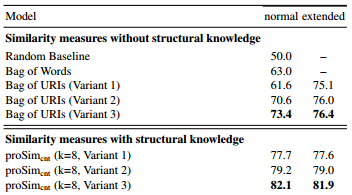
\includegraphics[scale=0.5]{img/lodifierevatab.png}
			\end{center}
		\end{frame}
		\begin{frame}{Precision - Recall}
			\begin{center}
				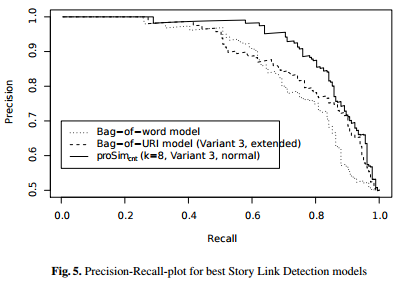
\includegraphics[scale=1]{img/lodifierevaplot.png}
			\end{center}
		\end{frame}
	\subsection{Conclusions}
		\begin{frame}{What to draw from this?}
			TODO
		\end{frame}			
		
		\begin{frame}{What we liked}
			\begin{itemize}
				\item full-text OIE
				\item uses many strengths of RDF
				\item relations arent overspecified
				\item extendable/improvable by improving/swapping Systems in the architecturesh
				\item Part of the LOD-Cloud
				\item results in standardized notation
				\item domain-independent
			\end{itemize}
		\end{frame}
		
		\begin{frame}{What we didnt like}
			\begin{itemize}
				\item Redundant processes like NER
				\item BlankNode Massacre
				\item confusing boxer relations not simplified for RDF (will be hard to search through)
				
				\vspace{15pt}
				
				\item Paper scratches only the surface of the system
				\item Some points are unclear / not even described
			\end{itemize}
		\end{frame}
\section{Conclusion}
	\begin{frame}{Weaknesses and Strengths of OIE}
		\begin{itemize}
			\item trades precision for recall
			\item OIE > IE if no sepcial task/domain is defined
			\item theory independent
			\item relations may be redundant/overspecified/unintended
			\item restricted usability of results due to low precision
		\end{itemize}
	\end{frame}
	\begin{frame}{Future Opportunities}
		\begin{itemize}
			\item better subsystems\\
				\begin{itemize}
					\item Coreference Resolution
					\item NER
					\item Disambiguation
				\end{itemize}
			\item improve semantic analysis
		\end{itemize}
	\end{frame}
	
	\begin{frame}[allowframebreaks]{References}
		A. Fader, S. Soderland, O. Etzioni. Identifying relations for open information extraction. Proc. of the Conf. on Empirical Methods in Natural Language, 2011\\
		\vspace{7pt}
		Augenstein, Isabelle, Sebastian Padó, and Sebastian Rudolph. "Lodifier: Generating linked data from unstructured text." The Semantic Web: Research and Applications. Springer Berlin Heidelberg, 2012. 210-224.\\
		\framebreak
		James R. Curran, Stephen Clark, and Johan Bos. 2007. Linguistically motivated large-scale NLP with C\&C and boxer. In Proceedings of the 45th Annual Meeting of the ACL on Interactive Poster and Demonstration Sessions (ACL '07). Association for Computational Linguistics, Stroudsburg, PA, USA, 33-36.\\
		\vspace{7pt}
	\end{frame}
\end{document}
